%!TEX root = ../main.tex

\chapter{Εισαγωγή}
\markboth{Εισαγωγή}{}

Στο κεφάλαιο αυτό γίνεται μια εισαγωγή στην κατάσταση που επικρατεί γύρω από τα άτομα με προβλήματα όρασης. Πιο συγκεκριμένα, παρατίθενται ορισμένα στατιστικά στοιχεία σχετικά με τον αριθμό των ατόμων με μειωμένη όραση, δίνεται ένας ορισμός της έννοιας της τύφλωσης και παρουσιάζονται μερικές από τις δυσκολίες που αναγκάζεται να αντιμετωπίσει ένα τέτοιο άτομο κατά την πλοήγησή του σε μια πόλη. Τέλος, αναφέρονται τα κίνητρα τα οποία με οδήγησαν στην συγγραφή αυτής της διπλωματικής εργασίας, ενώ παράλληλα δίνεται μια σύντομη περιγραφή των κεφαλαίων που την συνθέτουν.

\section{Στατιστικά στοιχεία για άτομα με προβλήματα όρασης}
Για να προχωρήσουμε στον σχεδιασμό ενός συστήματος πλοήγησης για τα άτομα με προβλήματα όρασης, πρέπει πρώτα να λάβουμε υπόψιν την κατηγοριοποίηση των ατόμων αυτών με βάση το ποσοστό τύφλωσής τους. Ο Παγκόσμιος Οργανισμός Υγείας (\url{https://www.who.int}), ο οποίος είναι ο πλέον αξιόπιστος φορέας σε θέματα που αφορούν την παγκόσμια υγεία, ορίζει την τύφλωση ως την μειωμένη ικανότητα όρασης σε βαθμό τέτοιο, ώστε τα προβλήματα δεν μπορούν να διορθωθούν με οποιοδήποτε μέσο, π.χ. γυαλιά, και παράλληλα προτείνει την ταξινόμηση των επιπέδων όρασης σε 4 βασικές κατηγορίες \cite{world_health_organization}:
\begin{itemize}
    \item Φυσιολογική όραση – Normal vision
    \item Μέτρια Διαταραχή όρασης – Moderate visual impairment
    \item Σοβαρή Διαταραχή όρασης – Severe visual impairment
    \item Ολική Απώλεια όρασης – Blindness
\end{itemize}

Σύμφωνα με μια έρευνα που δημοσιεύτηκε το 2017 \cite{bourne2017magnitude} το ποσοστό των ατόμων που παρουσιάζουν κάποιο πρόβλημα όρασης ή τύφλωση ανέρχεται στο 29,5\% επί του συνόλου του παγκόσμιου πληθυσμού, δηλαδή το 1/3 του πληθυσμού παρουσιάζει κάποια δυσλειτουργία στην όραση. Στη ίδια έρευνα αναφέρεται ότι 36 εκατομμύρια άνθρωποι πάσχουν από ολική τύφλωση, ενώ 217 εκατομμύρια παρουσιάζουν κάποιας μορφής σοβαρή ή ήπια πάθηση, ενώ αξίζει να σημειώσουμε ότι στις περισσότερες περιπτώσεις η απώλεια όρασης θα μπορούσε να είχε αποφευχθεί αν υπήρχε η κατάλληλη πρόληψη και διενέργεια οφθαλμολογικών εξετάσεων. Δεδομένου ότι το ποσοστό των ανθρώπων με κάποιας μορφής τύφλωση είναι υψηλότερο στις χώρες με μέτριο ή χαμηλό εισόδημα, καταλαβαίνουμε ότι η πρόληψη είναι άμεσα συνδεδεμένη με το βιοτικό επίπεδο των πολιτών και την οικονομική τους δυνατότητα για πρόσβαση σε ιατρική περίθαλψη.

\begin{figure}[H]
    \centering
    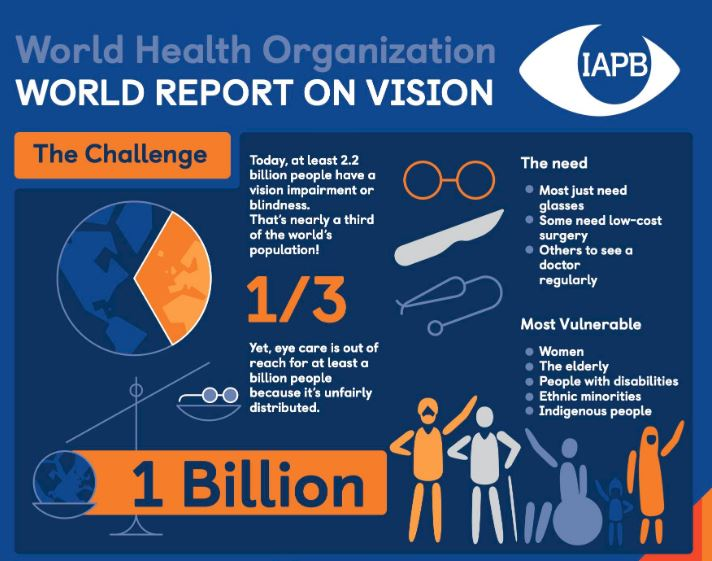
\includegraphics[width=0.8\textwidth]{images/who_stats.JPG}
    \caption{Έκθεση του Παγκόσμιου Οργανισμού Υγείας για τα ποσοστά ανθρώπων με προβλήματα όρασης \cite{Whatexac14:online}}
    \label{fig:who-stats}
\end{figure}

\section{Δυσκολίες πλοήγησης σε αστικά περιβάλλοντα}
Τα περισσότερα άτομα με προβλήματα όρασης επιλέγουν να ζήσουν σε πόλεις, επειδή η οργάνωση και οι δυνατότητες που τους παρέχονται είναι πολύ καλύτερες σε σύγκριση με τη ζωή στην ύπαιθρο. Παρ' όλα αυτά, ένα από τα μεγαλύτερα εμπόδια που αντιμετωπίζουν είναι αυτό της μετακίνησης. Η δυνατότητα αυτών των ατόμων να μετακινούνται αυτόνομα σε ένα αστικό περιβάλλον είναι αυτή που τους επιτρέπει να έχουν μια αξιοπρεπή ζωή, χωρίς αυτήν το βιοτικό τους επίπεδο μειώνεται δραματικά. Σύμφωνα με έρευνες που έχουν πραγματοποιηθεί σε αυτό το πεδίο \cite{riazi_outdoor_2016,parkin2012blind-needs}, μερικές από τις προκλήσεις που αντιμετωπίζουν τα άτομα με μειωμένη όραση είναι:
\begin{itemize}
    \item Συνεχής ανάγκη να ζητούν βοήθεια από περαστικούς
    \item Δυσκολία αναγνώρισης διαδρομών και χρήσης GPS
    \item Ρίσκο ατυχήματος
    \item Δυσκολία χρήσης των ανάγλυφων πλακιδίων για τυφλούς στα πεζοδρόμια
    \item Μη σωστή χρήση του λευκού μπαστουνιού οδηγεί σε ατυχήματα
    \item Φόβος χρήσης σκύλου-οδηγού
    \item Ελλιπής συντήρηση των πεζοδρομίων
    \item Απρόσεκτη συμπεριφορά πεζών
\end{itemize}

Ένα από τα σημαντικότερα προβλήματα μοιάζει να είναι η διάσχιση ενός δρόμου \cite{alwi2013survey}. Φανταστείτε τον εαυτό σας μπροστά από ένα μεγάλο σταυροδρόμι ή στην άκρη μιας μεγάλης λεωφόρου την οποία πρέπει να διασχίσετε. Ένα άτομο με μειωμένη όραση πρέπει να λάβει υπόψιν του πολλούς παράγοντες πριν ξεκινήσει να διασχίζει τον δρόμο, όπως για παράδειγμα την ύπαρξη ή όχι διάβασης πεζών, την ταχύτητα με την οποία πλησιάζουν τα διερχόμενα οχήματα, τυχόν εμπόδια που υπάρχουν κατά μήκος της διαδρομής του, καθώς επίσης και τον χρόνο τον οποίο χρειάζεται για να διασχίσει τον δρόμο.

Κατανοούμε λοιπόν την ανάγκη ύπαρξης καλύτερων υποδομών, σωστής και επαρκούς σήμανσης στους δρόμους, καθώς και την ανάγκη να γίνουμε πιο προσεκτικοί απέναντι στους συμπολίτες μας με μειωμένη όραση.

\section{Κίνητρα και σκοπός διπλωματικής εργασίας}
Ο βασικότερος λόγος που με ώθησε να ασχοληθώ με το συγκεκριμένο θέμα είναι η έλλειψη κατάλληλων προϋποθέσεων, ώστε τα άτομα με προβλήματα όρασης να έχουν ίσες ευκαιρίες στην καθημερινότητά τους και να μην περιορίζονται από το ποσοστό αναπηρίας που μπορεί να έχουν. Η καθημερινότητά μας καθορίζεται σε μεγάλο ποσοστό από το πόσο εύκολα μπορούμε να πραγματοποιήσουμε εργασίες αυτόνομα και ανεξάρτητα, χωρίς να βασιζόμαστε αποκλειστικά σε άλλους. Για τους πολίτες δίχως προβλήματα όρασης το να βγουν από το σπίτι τους και να μετακινηθούν μέχρι το πάρκο για μια βόλτα ή να περπατήσουν μέχρι το τοπικό σούπερ μάρκετ για τα ψώνια τους είναι κάτι το αυτονόητο και δεν αποτελεί επιπλέον κόπο. Αντιθέτως, για ένα άτομο με μειωμένη ή ολική απώλεια όρασης, ακόμα και το να βγει από το σπίτι του περπατώντας στην άκρη του πεζοδρομίου αποτελεί μια ενέργεια που ενέχει κινδύνους και απαιτεί έντονη συγκέντρωση και πνευματική προσπάθεια. Το δικαίωμα στην ελεύθερη, αυτόνομη και ασφαλή μετακίνηση είναι κάτι που θα έπρεπε να απολαμβάνουν όλοι οι άνθρωποι.

Η τεχνολογία σήμερα μας επιτρέπει να αλλάζουμε τον τρόπο με τον οποίο αντιμετωπίζουμε την πραγματικότητα και να δίνουμε λύσεις σε προβλήματα που είναι δύσκολα και περίπλοκα. Έχοντας υπόψιν τα παραπάνω, στόχος της παρούσας διπλωματικής εργασίας είναι ο σχεδιασμός και η υλοποίηση ενός συστήματος υποβοήθησης πλοήγησης που θα επιτρέπει στους χρήστες με προβλήματα όρασης να κινούνται με περισσότερη άνεση μέσα σε ένα αστικό περιβάλλον, συμβάλλοντας έτσι στην αύξηση της αυτονομίας τους. Θα πρέπει να τονιστεί ότι το προτεινόμενο σύστημα στόχο έχει να ενισχύσει την λειτουργία του λευκού μπαστουνιού, που χρησιμοποιείται κατά κόρον από τους τυφλούς, και όχι να την αντικαταστήσει. Παράλληλα, η παρούσα εργασία εστιάζει κυρίως στην παροχή βοήθειας στους χρήστες για την αποτελεσματικότερη και ασφαλέστερη διάσχιση μιας διάβασης πεζών, ενώ αξίζει να τονιστεί ότι η παροχή ανατροφοδότησης στον χρήστη κατά την πλοήγηση δίνεται μέσω της αφής, με σκοπό την αξιοποίηση του απτικού καναλιού και την μείωση του φόρτου στο κανάλι της ακοής.

\section{Διάρθρωση διπλωματικής εργασίας}
Έχοντας επίγνωση των αναγκών και της πολυπλοκότητας ενός συστήματος πλοήγησης για άτομα με προβλήματα όρασης, έχει γίνει προσπάθεια να παρουσιαστούν με τον πιο κατανοητό και περιεκτικό τρόπο όλες οι πλευρές ενός τέτοιου συστήματος. Για τον λόγο αυτό η παρούσα εργασία διαμορφώνεται ως εξής:
\begin{itemize}
    \item Στο κεφάλαιο 2 «\nameref{ch:state-of-the-art}» γίνεται αναφορά στην προγενέστερη έρευνα που έχει γίνει στο αντίστοιχο ερευνητικό πεδίο. Πιο συγκεκριμένα, παρουσιάζονται τα βοηθητικά μέσα που έχουν στη διάθεσή τους τα άτομα με δυσκολία όρασης, γίνεται διαχωρισμός των ηλεκτρονικών συστημάτων υποβοήθησης πλοήγησης σε τρεις κύριες κατηγορίες και τέλος παρατίθενται μερικά από τα πιο αντιπροσωπευτικά συστήματα πλοήγησης εξωτερικού χώρου που έχουν αναπτυχθεί.
    \item Στο κεφάλαιο 3 «\nameref{ch:system-architecture}» γίνεται μια αναλυτική περιγραφή της αρχιτεκτονικής του προτεινόμενου συστήματος, των ελάχιστων προδιαγραφών ενός συστήματος πλοήγησης για άτομα με προβλήματα όρασης και παρουσιάζονται με λεπτομέρεια τα διάφορα μέρη που χρησιμοποιήθηκαν για την υλοποίησή του. 
    \item Στο κεφάλαιο 4 «\nameref{ch:demo}» παρουσιάζεται ο τρόπος με τον οποίο έγινε ο πειραματικός έλεγχος της ορθής λειτουργίας του συστήματος και αναφέρονται τα διάφορα αποτελέσματα που προέκυψαν.
    \item Στο κεφάλαιο 5 «\nameref{ch:conclusion}» αναλύονται τα πλεονεκτήματα και τα μειονεκτήματα του προτεινόμενου συστήματος και παρατίθενται διάφορες προτάσεις για την βελτίωση της αποδοτικότητάς του.
\end{itemize}